\documentclass{beamer}

\mode<presentation>
\usepackage{amsmath,amssymb,mathtools}
\usepackage{textcomp}
\usepackage{gensymb}
\usepackage{adjustbox}
\usepackage{subcaption}
\usepackage{enumitem}
\usepackage[utf8]{inputenc}
\usepackage{amssymb}
\usepackage{newunicodechar}
\usepackage{enumitem}
\setlist{nosep} % optional: removes vertical gaps
\setlist[enumerate]{label=\arabic*)} % custom numbering if you want

\newunicodechar{√}{$\sqrt{\;}$}
\newunicodechar{✅}{\checkmark}
\newunicodechar{❌}{\texttimes}
\usepackage{multicol}
\usepackage{listings}
\usepackage{url}
\usepackage{graphicx} % <-- needed for images
\def\UrlBreaks{\do\/\do-}

\usetheme{Boadilla}
\usecolortheme{lily}
\setbeamertemplate{footline}{
  \leavevmode%
  \hbox{%
  \begin{beamercolorbox}[wd=\paperwidth,ht=2ex,dp=1ex,right]{author in head/foot}%
    \insertframenumber{} / \inserttotalframenumber\hspace*{2ex}
  \end{beamercolorbox}}%
  \vskip0pt%
}
\setbeamertemplate{navigation symbols}{}

\lstset{
  frame=single,
  breaklines=true,
  columns=fullflexible,
  basicstyle=\ttfamily\tiny   % tiny font so code fits
}

\numberwithin{equation}{section}

% ---- your macros ----
\providecommand{\nCr}[2]{\,^{#1}{#2}}
\providecommand{\nPr}[2]{\,^{#1}P_{#2}}
\providecommand{\mbf}{\mathbf}
\providecommand{\pr}[1]{\ensuremath{\Pr\left(#1\right)}}
\providecommand{\qfunc}[1]{\ensuremath{Q\left(#1\right)}}
\providecommand{\sbrak}[1]{\ensuremath{{}\left[#1\right]}}
\providecommand{\lsbrak}[1]{\ensuremath{{}\left[#1\right.}}
\providecommand{\rsbrak}[1]{\ensuremath{\left.#1\right]}}
\providecommand{\brak}[1]{\ensuremath{\left(#1\right)}}
\providecommand{\lbrak}[1]{\ensuremath{\left(#1\right.}}
\providecommand{\rbrak}[1]{\ensuremath{\left.#1\right)}}
\providecommand{\cbrak}[1]{\ensuremath{\left\{#1\right\}}}
\providecommand{\lcbrak}[1]{\ensuremath{\left\{#1\right.}}
\providecommand{\rcbrak}[1]{\ensuremath{\left.#1\right\}}}
\theoremstyle{remark}
\newtheorem{rem}{Remark}
\newcommand{\sgn}{\mathop{\mathrm{sgn}}}
\providecommand{\abs}[1]{\left\vert#1\right\vert}
\providecommand{\res}[1]{\Res\displaylimits_{#1}}
\providecommand{\norm}[1]{\lVert#1\rVert}
\providecommand{\mtx}[1]{\mathbf{#1}}
\providecommand{\mean}[1]{E\left[ #1 \right]}
\providecommand{\fourier}{\overset{\mathcal{F}}{ \rightleftharpoons}}
\providecommand{\system}{\overset{\mathcal{H}}{ \longleftrightarrow}}
\providecommand{\dec}[2]{\ensuremath{\overset{#1}{\underset{#2}{\gtrless}}}}
\newcommand{\myvec}[1]{\ensuremath{\begin{pmatrix}#1\end{pmatrix}}}
\let\vec\mathbf
% ---------------------

\title{Matgeo Presentation - Problem 4.10.23}
\author{ee25btech11021 - Dhanush sagar}

\begin{document}
	

		




%---------------- Title Page ----------------
\begin{frame}
  \titlepage
\end{frame}

%---------------- Problem Statement ----------------
\begin{frame}{Problem Statement}
Find the equation of the line passing through the point of intersection of 2x + y = 5
and x + 3y + 8 = 0 and parallel to the line 3x + 4y = 7.
\end{frame}

%---------------- Mathematical Formula ----------------
\begin{frame}{solution}

The two given lines are written in matrix form as
\begin{align}
l_1 = \myvec{2 \\ 1}\vec{x} &= 5, \\
l_2 = \myvec{1 \\ 3}\vec{x} &= -8.\\
l_3 = \myvec{3 \\ 4}\vec{x} &= 7. \\
\end{align}
\noindent{\small Normals and constants for the given lines $l_1$ and $l_2$.}
\begin{align}
\vec{n}_1 &= \myvec{2\\1}, \quad c_1=5 \\
\vec{n}_2 &= \myvec{1\\3}, \quad c_2=-8
\end{align}
\noindent{\small General family of lines through the intersection, written as $l_1+\lambda l_2$.}
\end{frame}
\begin{frame}{solution}
\begin{align}
(\vec{n}_1^T\vec{x}-c_1) + \lambda(\vec{n}_2^T\vec{x}-c_2) &= 0
\end{align}

\noindent{\small Explicit expanded form of the family of lines.}
\begin{align}
\myvec{2 & 1}\vec{x}-5 + \lambda\big(\myvec{1 & 3}\vec{x}+8\big) &= 0 \\
\implies \myvec{2+\lambda & 1+3\lambda}\vec{x} &= 5 - 8\lambda.  
\end{align}



Normal of the line $l_3$, to which our required line must be parallel.


\begin{align}
\vec{m} &= \myvec{3\\4}
\end{align}

\noindent{\small Normal vector of the family of lines.}

\begin{align}
\vec{N}(\lambda) &= \vec{n}_1 + \lambda\vec{n}_2 = \myvec{2+\lambda\\1+3\lambda}
\end{align}
\end{frame}
\begin{frame}{solution}
\noindent{\small Condition for parallelism with $\vec{m}$.}
\begin{align}
\vec{N}(\lambda) &= \alpha\vec{m}
\implies \myvec{2+\lambda\\1+3\lambda} = \alpha\myvec{3\\4}
\end{align}

\noindent{\small Solve these equations to determine $\lambda$.}

\begin{align}
3\alpha - \lambda &= 2 \\
4\alpha - 3\lambda &= 1
\end{align}
augmented matrix 
\begin{align}
\myvec{3 & -1 & \vline & 2 \\ 4 & -3 & \vline & 1}
\end{align}

\begin{align}
R_1 &\to \tfrac{1}{3}R_1 \\
\myvec{3 & -1 & \vline & 2 \\ 4 & -3 & \vline & 1} 
&\;\Rightarrow\;
\myvec{1 & -\tfrac{1}{3} & \vline & \tfrac{2}{3} \\ 4 & -3 & \vline & 1}
\end{align}

\begin{align}
R_2 &\to R_2 - 4R_1 \\
\myvec{1 & -\tfrac{1}{3} & \vline & \tfrac{2}{3} \\ 4 & -3 & \vline & 1}
&\;\Rightarrow\;
\myvec{1 & -\tfrac{1}{3} & \vline & \tfrac{2}{3} \\ 0 & -\tfrac{5}{3} & \vline & -\tfrac{5}{3}}
\end{align}

\begin{align}
R_2 &\to \left(-\tfrac{3}{5}\right)R_2 \\
\myvec{1 & -\tfrac{1}{3} & \vline & \tfrac{2}{3} \\ 0 & -\tfrac{5}{3} & \vline & -\tfrac{5}{3}}
&\;\Rightarrow\;
\myvec{1 & -\tfrac{1}{3} & \vline & \tfrac{2}{3} \\ 0 & 1 & \vline & 1}
\end{align}

\begin{align}
R_1 &\to R_1 + \tfrac{1}{3}R_2 \\
\myvec{1 & -\tfrac{1}{3} & \vline & \tfrac{2}{3} \\ 0 & 1 & \vline & 1}
&\;\Rightarrow\;
\myvec{1 & 0 & \vline & 1 \\ 0 & 1 & \vline & 1}
\end{align}
\end{frame}
\begin{frame}{solution}
\begin{align}
\lambda &= 1
\end{align}

substituting value of $\lambda$ in eq(0.9) .Final equation of the required line in matrix form.
\begin{align}
\myvec{3 & 4}\vec{x} + 3 &= 0
\end{align}
\end{frame}
%---------------- C Source Code ----------------
\begin{frame}[fragile]{C Source Code:line generator.c}
\begin{verbatim}
/* line_generator.c */
#include <stdio.h>
/* Generate points along line N^T x + c = 0
   Nx, Ny = components of normal vector
   c = constant
   tmin, tmax = steps along direction perpendicular to N
*/
void generate_line_points(double Nx, double Ny, double c, int tmin, int tmax) {
    double dx = -Ny;  // direction vector perpendicular to normal
    double dy = Nx;
// Pick a point on the line: x0 = 0, y0 = -c/Ny
    double x0 = 0.0;
    double y0 = -c / Ny;
    for (int t = tmin; t <= tmax; t++) {
        double x = x0 + t*dx;
        double y = y0 + t*dy;
        printf("%.6f %.6f\n", x, y);
    }
}



\end{verbatim}
\end{frame}

%---------------- Python solve.py ----------------
\begin{frame}[fragile]{Python Script:solve matrix line.py}
\begin{verbatim}
import ctypes
import numpy as np

# --- Step 0: Load C library ---
lib = ctypes.CDLL("./line_generator.so")
lib.generate_line_points.argtypes = [ctypes.c_double, ctypes.c_double, ctypes.c_double,
                                     ctypes.c_int, ctypes.c_int]

# --- Step 1: Matrix method to find required line ---
n1 = np.array([2, 1])
c1 = 5
n2 = np.array([1, 3])
c2 = -8
n3 = np.array([3, 4])  # line to be parallel



\end{verbatim}
\end{frame}
\begin{frame}[fragile]{Python Script:solve matrix line.py}
\begin{verbatim}
# Family of lines: N(lambda) = n1 + lambda*n2
# Parallel condition: N(lambda) = alpha * n3
# Solve for lambda:
lambda_val = 1  # from calculation
# Normal vector and constant of required line
N = n1 + lambda_val * n2
c = c1 + lambda_val * c2

print("Normal vector of required line:", N)
print("Constant term:", c)
print(f"Equation of line: {N[0]}x + {N[1]}y + {c} = 0\n")

# --- Step 2: Call C function to generate points ---
print("Points on the line:")
lib.generate_line_points(float(N[0]), float(N[1]), float(c), 
-5, 5)
\end{verbatim}
\end{frame}

\begin{frame}[fragile]{Python Script: plot matrix line.py}
\begin{verbatim}
import numpy as np
import matplotlib.pyplot as plt
# --- Step 1: Matrix method to find required line ---
n1 = np.array([2, 1])
c1 = 5
n2 = np.array([1, 3])
c2 = -8
n3 = np.array([3, 4])  # line to be parallel
lambda_val = 1  # from calculation
# Normal vector and constant of required line
N = n1 + lambda_val * n2
c = c1 + lambda_val * c2
print("Normal vector of required line:", N)
print("Constant term:", c)
print(f"Equation of line: {N[0]}x + {N[1]}y + {c} = 0\n")
# --- Step 2: Generate points along the line in Python ---
d = np.array([-N[1], N[0]])


\end{verbatim}
\end{frame}
\begin{frame}[fragile]{Python Script: plot lines plane.py}
\begin{verbatim}
t_values = np.linspace(-10, 10, 21)  # 21 points
# Pick a point on the line: x0 = 0, y0 = -c/N[1]
x0 = 0
y0 = -c / N[1]
points = np.array([ [x0 + t*d[0], y0 + t*d[1]] for t in t_values ])
# --- Step 3: Plot ---
plt.figure(figsize=(8,6))
plt.scatter(points[:,0], points[:,1], color='red', label='Generated points')
# Plot the exact line
x_vals = np.linspace(points[:,0].min()-1, points[:,0].max()+1, 100)
y_vals = -(N[0]*x_vals + c)/N[1]
plt.plot(x_vals, y_vals, label='Required line', color='blue')
plt.xlabel('x')
plt.ylabel('y')
plt.title('Line generated using matrix method')
plt.grid(True)
plt.legend() plt.axis('equal') plt.show()


\end{verbatim}
\end{frame}

%---------------- Result Plot ----------------
\begin{frame}{Result Plot}
 \begin{figure}[H]
     \centering
     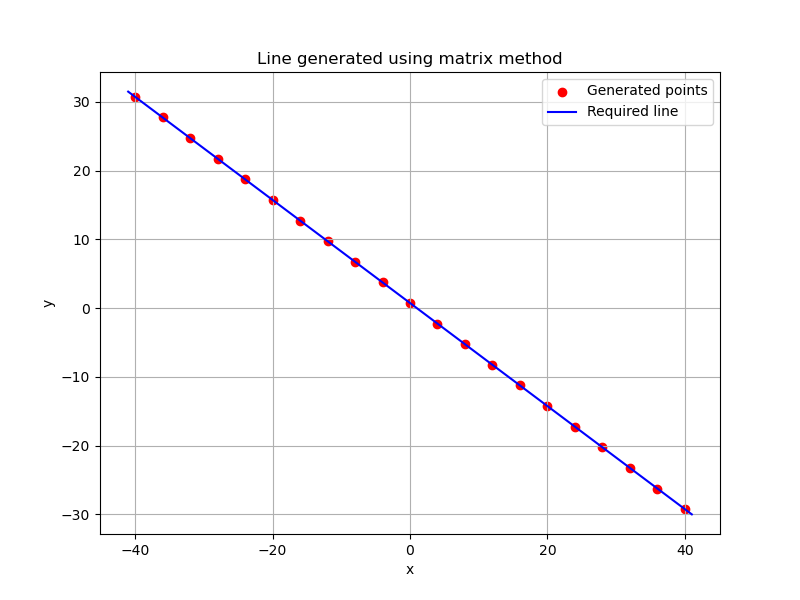
\includegraphics[width=0.7\columnwidth]{figs/fig1.png}
     \caption*{}
     \label{fig:fig1}
 \end{figure}
 
\end{frame}

\end{document}
\end{document}
